\documentclass[tikz,border=8pt]{standalone}

\usepackage[T1]{fontenc}
\usepackage[utf8]{inputenc}
\usepackage{lmodern}
\usetikzlibrary{arrows.meta,fit,positioning,backgrounds}

\definecolor{distBlue}{RGB}{30,90,200}
\definecolor{varRed}{RGB}{176,20,30}
\definecolor{cvarFill}{RGB}{252,190,190}
\definecolor{idleFill}{RGB}{236,236,236}

\begin{document}
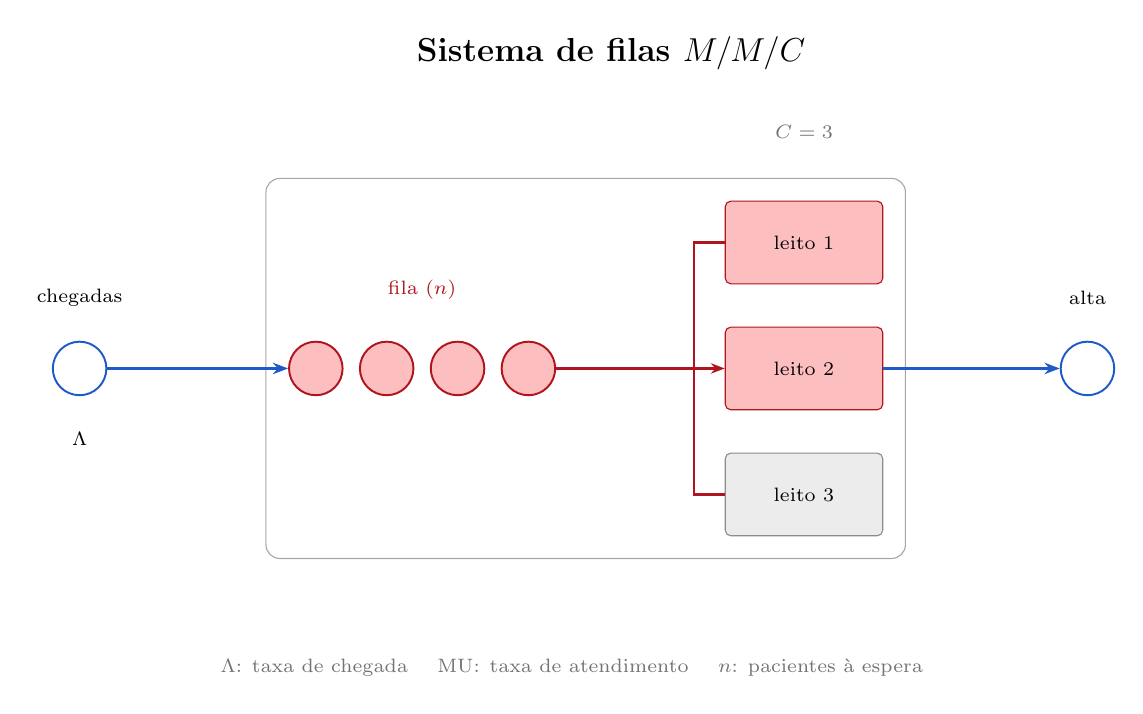
\begin{tikzpicture}[
  font=\small,
  >=Stealth,
  pac/.style={
    circle,
    draw=distBlue,
    fill=white,
    inner sep=0pt,
    minimum size=6.8mm,
    font=\scriptsize,
    line width=0.7pt,
  },
  pachot/.style={
    pac,
    draw=varRed,
    fill=cvarFill,
  },
  leito/.style={
    draw=black!45,
    rounded corners=2pt,
    minimum width=20mm,
    minimum height=10.5mm,
    align=center,
    font=\scriptsize,
    inner sep=2pt,
  },
]

  \node[font=\bfseries\large] at (7.1,7.55)
    {Sistema de filas $M/M/C$};

  \node[pac] (in) at (0.35,3.55) {};
  \node[font=\scriptsize] at (0.35,4.45) {chegadas};
  \node[font=\scriptsize] at (0.35,2.65) {$\Lambda$};

  \node[pachot] (q1) at (3.35,3.55) {};
  \node[pachot] (q2) at (4.25,3.55) {};
  \node[pachot] (q3) at (5.15,3.55) {};
  \node[pachot] (q4) at (6.05,3.55) {};
  \node[font=\scriptsize, varRed] at (4.7,4.55) {fila ($n$)};

  \node[leito, fill=cvarFill, draw=varRed] (s1) at (9.55,5.15) {leito 1};
  \node[leito, fill=cvarFill, draw=varRed] (s2) at (9.55,3.55) {leito 2};
  \node[leito, fill=idleFill] (s3) at (9.55,1.95) {leito 3};
  \node[font=\scriptsize, text=black!55] at (9.55,6.55) {$C=3$};

  \node[pac] (out) at (13.15,3.55) {};
  \node[font=\scriptsize] at (13.15,4.45) {alta};

  \begin{scope}[on background layer]
    \node[draw=black!35, rounded corners=5pt, inner sep=8pt,
          fit=(q1)(q4)(s1)(s3)] (sys) {};
  \end{scope}

  \draw[-{Stealth[length=5.5pt]}, distBlue, line width=0.95pt]
    (in) -- (q1);
  \coordinate (bus) at (8.15,3.55);
  \draw[varRed, line width=0.8pt] (q4) -- (bus);
  \draw[varRed, line width=0.8pt] (bus) |- (s1.west);
  \draw[-{Stealth[length=5pt]}, varRed, line width=0.8pt] (bus) -- (s2.west);
  \draw[varRed, line width=0.8pt] (bus) |- (s3.west);
  \draw[-{Stealth[length=5.5pt]}, distBlue, line width=0.95pt]
    (s2.east) -- (out);

  \node[font=\scriptsize, text=black!55] at (6.6,-0.25)
    {$\Lambda$: taxa de chegada
     \quad $\mathrm{MU}$: taxa de atendimento
     \quad $n$: pacientes \`a espera};

\end{tikzpicture}
\end{document}
